\section{Nota Teórica}

A continuación se muestra un diagrama del diseño general de la placa:
\begin{figure}[H]
    \centering
    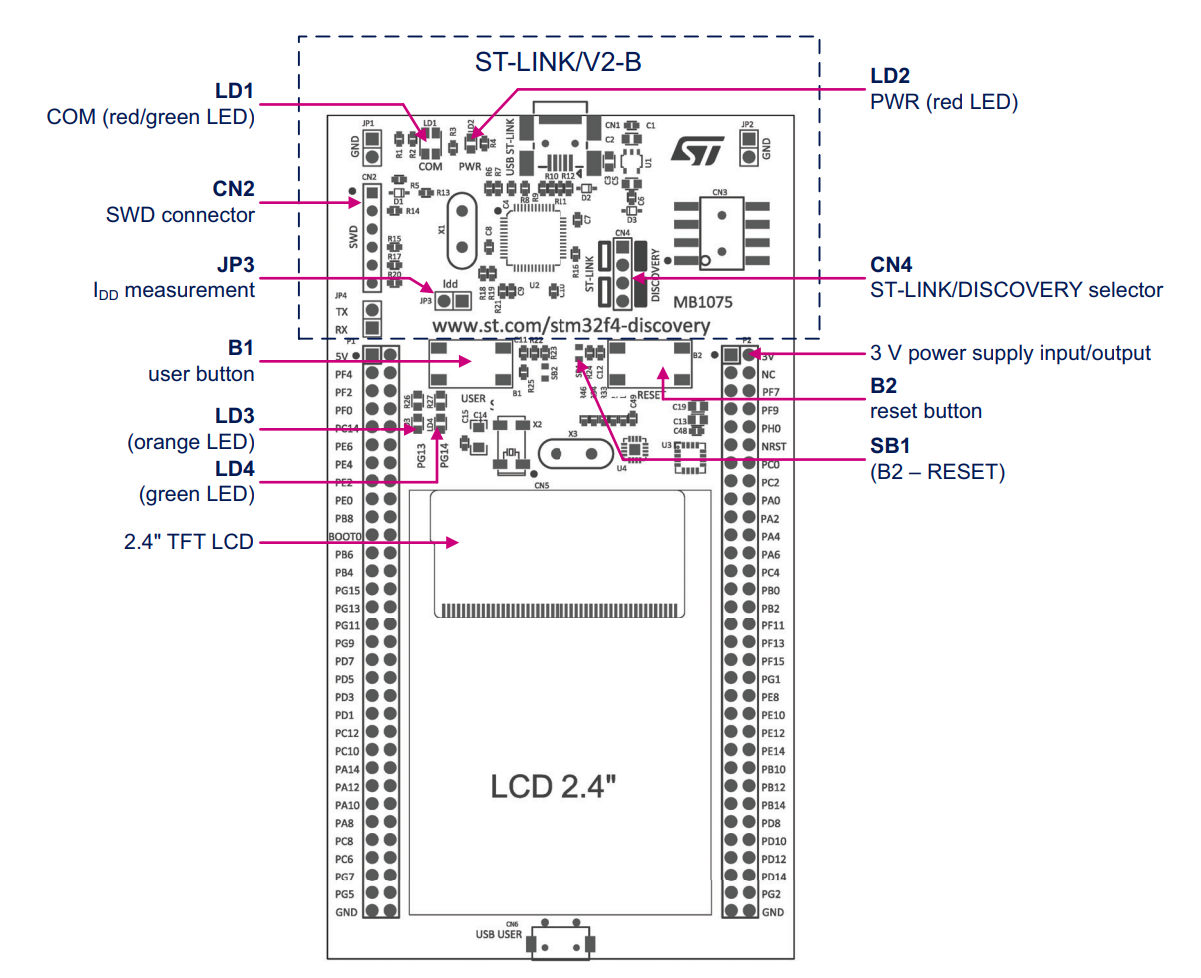
\includegraphics[scale=.5]{Imagenes/layout.png}
    \caption{Diseño general del STM32F429i Discovery Kit \cite{discovery}}
    \label{fig:diag_general}
\end{figure}

\subsection{Componentes empleados.}
La siguiente tabla detalla los componentes y la cantidad utilizada.
\begin{center}
    \begin{tabular}{|c|c|}
        \hline
         Componente & Cantidad\\ \hline
         STM32F429i Discovery Kit & 1\\
         Bateria 9V & 1 \\
         Resistencia 10k$\Omega$ & 2 \\
         Resistencia 2.2k$\Omega$ & 1 \\ \hline
    \end{tabular}
\end{center}

\subsection{STM32F429ZI}
La siguiente datos de la placa STM32F429 Discovery kit fueron tomados de la hoja de datos oficial del fabricante \cite{discovery}.
La placa STM32F429 Discovery kit se basa en el microcontrolador STM32F429ZI, el cual es un microcontrolador de alto rendimiento de la serie STM32F4 desarrollado por STMicroelectronics, basado en el núcleo ARM Cortex-M4. Este procesador está diseñado para aplicaciones de tiempo real que requieren cálculos intensivos y alto control sobre periféricos. A continuación, se detalla su arquitectura, características clave del procesador, y el uso de registros.
El procesador ARM Cortex-M4 integrado en el STM32F429ZI opera a una frecuencia de 180 MHz. Este procesador incorpora una Unidad de Punto Flotante (FPU) compatible con el estándar IEEE 754, lo que permite realizar operaciones de punto flotante de forma rápida y eficiente. Además, incluye una caché de instrucciones y datos (I/D), que optimiza la velocidad de acceso a memoria y minimiza las latencias durante la ejecución del código.
El Cortex-M4 soporta procesamiento digital de señales (DSP), incorporando instrucciones SIMD (Single Instruction Multiple Data), que mejoran el rendimiento en algoritmos matemáticos, como filtros y procesamiento de señales, aumentando la eficiencia del sistema. Ofrece un sistema de gestión de interrupciones capaz de manejar hasta 240 interrupciones con 16 niveles de prioridad. Estas interrupciones son gestionadas por el NVIC (Nested Vectored Interrupt Controller), asegurando respuestas rápidas y eficientes a eventos de hardware software críticos.
El microcontrolador dispone de 2 MB de memoria Flash interna, utilizada para almacenar el firmware y las aplicaciones críticas. Esta memoria permite múltiples ciclos de lectura y escritura, garantizando la estabilidad del sistema durante las actualizaciones. Además, cuenta con 256 KB de SRAM interna para la ejecución de tareas en tiempo real. Para aplicaciones que requieren un manejo intensivo de datos, como el procesamiento de señales, el sistema puede hacer uso de una memoria externa SDRAM de 64 Mbits, útil para almacenamiento temporal y creación de buffers.
El STM32F429ZI ofrece varios puertos GPIO (General Purpose I/O), los cuales se configuran a través de registros específicos para definir su modo de operación, ya sea como entrada, salida, función alternativa o analógica.
El microcontrolador dispone de hasta 14 temporizadores, algunos de ellos con funciones avanzadas como la generación de PWM (Pulse Width Modulation). Cada temporizador se gestiona mediante los registros de control de temporizadores.

\subsection{Giroscopio y pantalla LCD}
La interfaz SPI permite la comunicación entre el microcontrolador y el giroscopio MEMS I3G4250D.
El giroscopio MEMS I3G4250D integrado en la placa es un sensor de movimiento de tres ejes que permite medir la velocidad angular en rangos ajustables de ±245, ±500 o ±2000 grados por segundo (dps), lo que lo hace adecuado para aplicaciones de monitoreo de vibraciones y detección de movimientos sísmicos. Este giroscopio cuenta con una interfaz de salida digital compatible con SPI e I2C, lo que facilita su integración con el microcontrolador y permite la captura eficiente de datos en tiempo real. Además, el I3G4250D incluye un filtro pasa bajos configurable que mejora la precisión en la medición de cambios de orientación y detecta variaciones sutiles en el movimiento en los ejes X, Y y Z.
La pantalla LCD TFT integrada es de 2.4 pulgadas con una resolución QVGA de 240 x 320 píxeles y es capaz de mostrar hasta 262,000 colores. Es controlada mediante un controlador ILI9341 a través de un protocolo RGB, esta pantalla facilita la visualización de información como el nivel de batería, los datos de los ejes del giroscopio y el estado de la comunicación USART/USB. Además, su bajo consumo de energía y compatibilidad con voltajes típicos de 2.8 V la hacen ideal para aplicaciones en sistemas portátiles.

\subsection{ThingsBoard}
ThingsBoard es una plataforma de Internet de las Cosas (IoT) de código abierto que permite recopilar, procesar y visualizar datos en tiempo real desde dispositivos y sensores conectados. Facilita la administración remota y el monitoreo de dispositivos IoT, ofreciendo herramientas avanzadas para crear visualizaciones interactivas, analizar datos y generar alertas según condiciones específicas.
Entre sus características principales se encuentra la gestión de dispositivos, que permite registrar y controlar dispositivos IoT de manera eficiente. Cada dispositivo puede configurarse para enviar datos en intervalos regulares o cuando ocurren eventos específicos, utilizando protocolos de comunicación como MQTT, HTTP y CoAP, lo cual permite una fácil integración con diversos dispositivos.
ThingsBoard también permite el procesamiento y almacenamiento de datos a gran escala en tiempo real, aplicando reglas de procesamiento para ejecutar acciones basadas en eventos, como activar alertas o enviar datos a servicios en la nube cuando se cumplen condiciones específicas. Permite crear dashboards personalizables con widgets interactivos como gráficos de líneas, medidores, tablas y mapas, facilitando el análisis y la monitorización de datos en tiempo real.
La plataforma permite configurar alertas y notificaciones basadas en reglas definidas por el usuario, ideal para aplicaciones que requieren alertas inmediatas en situaciones críticas, como baja batería o detección de actividad sísmica. Estas notificaciones pueden enviarse por correo electrónico o integrarse con otros sistemas de mensajería en tiempo real.
Diseñada para aplicaciones de cualquier escala, ThingsBoard es altamente escalable y cuenta con características de seguridad avanzadas que incluyen autenticación de dispositivos, control de acceso basado en roles y cifrado de datos. \cite{things}
En este laboratorio, ThingsBoard se utilizará para recibir y visualizar datos del giroscopio y el nivel de batería de la placa STM32F429 Discovery Kit. Un script en Python enviará estos datos a la plataforma, representándolos en un dashboard interactivo para observar en tiempo real las variaciones de movimiento y el estado de la energía. Además, las alertas configuradas en ThingsBoard enviarán notificaciones en caso de batería baja, garantizando una respuesta rápida ante condiciones críticas.



